\documentclass[UTF8,11pt]{beamer}

\usepackage[utf8]{inputenc}
\usepackage{latexsym}
\usepackage[T1]{fontenc}
\usepackage{lmodern}
\usepackage[english]{babel}
\usepackage{amsmath}
\usepackage{amsfonts}
\usepackage{amssymb}
\usepackage{graphicx}
\usepackage{tikz}
\usetikzlibrary{matrix,shapes,arrows,positioning,fit,backgrounds,calc}
\usepackage{overpic}
\usepackage[]{algorithm}
\usepackage[]{algpseudocode} % noend
\usepackage[most]{tcolorbox}
\usepackage{ulem}
\usepackage{fancybox}
\usetikzlibrary{decorations.pathreplacing}
\usetheme{Eastlansing}
\newcommand{\fallingfactorial}[1]{%
	^{\underline{#1}}%
}
\mode<presentation>
\begin{document}
	\author{MA Jun}
	\title{Problem Solving}
	\subtitle{2-12 Hashing}
	\logo{
\includegraphics[width=0.05\textwidth]{../figs/ICS_LOGO_left.png}}
	\institute{Institute of Computer Software}
	%\date{March 31, 2020}
	%\subject{}
	%\setbeamercovered{transparent}
	%\setbeamertemplate{navigation symbols}{}
\begin{frame}[plain]
	\maketitle
\end{frame}
\begin{frame}           %生成目录页,目录太长时加选项[shrink]
	\addtocounter{framenumber}{-2}%---------位置放在beginframe之后,不然无效
	\frametitle{Contents}
	\thispagestyle{empty}
	\tableofcontents[hideallsubsections]
\end{frame}
\AtBeginSection[]{
	\begin{frame}           %生成目录页,目录太长时加选项[shrink]
		\addtocounter{framenumber}{-1}%---------位置放在beginframe之后,不然无效
		\frametitle{Contents}
		\thispagestyle{empty}
		\tableofcontents[currentsection,hideallsubsections]
	\end{frame}
}

\begin{frame}
\frametitle{Applications of Hashing}
There are many applications of hashing \blue{(not limited to hash table)}, including modern day cryptography hash functions. Some of these applications are listed below:
\begin{itemize}
	\item Message Digest
	\item Password Verification
	\item Data Structures (Programming Languages)
	\item Compiler Operation
	\item Rabin-Karp Algorithm
	\item Linking File Name and Path Together
\end{itemize}
{\tiny
	\href{https://www.geeksforgeeks.org/applications-of-hashing/}{https://www.geeksforgeeks.org/applications-of-hashing/}
}
\end{frame}

\section{Hash-table: Basic Idea}


\begin{frame}
\begin{block}{}
	\begin{center}
		Many applications require a \textbf{\red{Dynamic Set}} that supports only the \textbf{\blue{dictionary}} operations \teal{\textproc{Insert}}, \teal{\textproc{Search}}, and \teal{\textproc{Delete}}.
	\end{center}
\end{block}
\pause
\begin{block}{}
	\begin{center}
 	Searching for an element in a hash table can take as long as searching for an element in a linked list— \teal{$\Theta(n)$} time in the \blue{worst case}. 
	\end{center}
\end{block}
\pause
\begin{block}{}
	\begin{center}
	 Under reasonable assumptions, the \blue{average time} to search for an element in a hash table is \teal{$\Theta(1)$}.
	\end{center}
\end{block}
\end{frame}

\begin{frame}
\frametitle{Hashing: the idea}
\begin{center}
	\question{}{ When should we use hash table? 
		
		What situations is the hash table suitable for?}

	\begin{tikzpicture}
		\pause
		\node (b) at (4,0){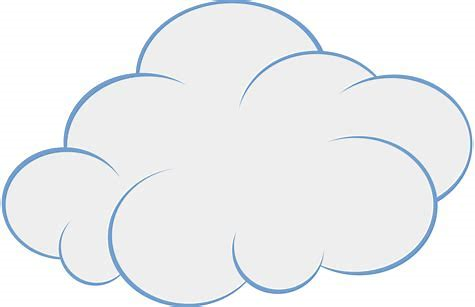
\includegraphics[width=4cm]{figs/cloud.png}};
		\node at(4,-0.5) [color=blue]{Key Space};
		
		\pause
		\fill[ball color=red!60] (3,0.5) circle (0.1)node(x)[above,right]{$x$};
		\node at (4,2) [fill= yellow,text width=4cm]{\footnotesize{Very \red{large}, but only a \red{small part} is used in an application at a certain time.}};
		
		
		\pause
		\foreach \y in{2,1.5,-1.5,-2}:
			\draw (-4,\y-0.25) rectangle (-3,\y+0.25); 
		\draw (-4,-0.25) rectangle node(k){ } (-3,0.25); 
		\draw (-4,0.25) rectangle node{$\cdots$} (-3,1.25); 
		\draw (-4,-0.25) rectangle node{$\cdots$} (-3,-1.25); 
		\node at(-5,2){$E\left[0\right]$};
		\node at(-5,1.5){$E\left[1\right]$};		
		\node at(-5,-2){$E\left[m-1\right]$};
		\node at (-4,3) [fill= yellow]{\footnotesize{Feasible size}};
		
		\pause
		\node (a)[color=black, draw,rectangle,fill=gray] at(-0.5,0) {Hash Function} ;
		
		\draw [dashed,color=red,thick,->](x)--(a);
		\draw [dashed,color=red,thick,->](a)--(k);
		\node at(-5,0){$E\left[{\color{red}k}\right]$};

		\pause				
		\node at (-0.5,1.5) [fill= yellow,text width=4cm]{\footnotesize{
				\begin{itemize}
				\item Index distribution
				\item Collision handling
				\end{itemize}
			}
		};
	\end{tikzpicture}
\end{center}
\end{frame}


\begin{frame}
\frametitle{Hashing: the idea}
\begin{center}
	\question{}{ What is a Collision? When does it take place?}

	\pause
	\begin{tikzpicture}
	\filldraw [fill=gray](-2,-1) rectangle (1,1);
	\node (a)[color=black] at(-0.5,0) {Hash Function} ;

	\node (b) at (4,0){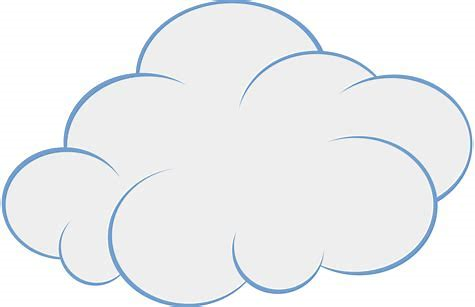
\includegraphics[width=4cm]{figs/cloud.png}};
	\node at(4,-0.5) [color=blue]{Key Space};

	
	
	
	\foreach \y in{2,1.5,-1.5,-2}:
	\draw (-4,\y-0.25) rectangle (-3,\y+0.25); 
	\draw (-4,-0.25) rectangle node(k){ } (-3,0.25); 
	\draw (-4,0.25) rectangle node{$\cdots$} (-3,1.25); 
	\draw (-4,-0.25) rectangle node{$\cdots$} (-3,-1.25); 
	\node at(-5,2){$E\left[0\right]$};
	\node at(-5,1.5){$E\left[1\right]$};		
	\node at(-5,-2){$E\left[m-1\right]$};
	
	\pause
	\fill[ball color=red!60] (3,0.5) circle (0.1)node(x)[above,right]{$x$};
	\fill[ball color=red!60] (2.5,-0.2) circle (0.1)node(y)[above,right]{$y$};
	
	\pause
	\node at(-5,0){$E\left[{\color{red}k}\right]$};
	\draw [dashed,color=red,thick,->](x)--(k);
	\draw [dashed,color=red,thick,->](y)--(k);
	\end{tikzpicture}
\end{center}
\end{frame}

\begin{frame}
\frametitle{Collision}
\begin{center}
	\question{}{Given $n$ keys and $m$ slots, what is the expected number of keys hashed into the same slot? }
	\begin{tikzpicture}
	\filldraw [fill=gray](-2,-1) rectangle (1,1);
	\node (a)[color=black] at(-0.5,0) {Hash Function} ;
	
	\node (b) at (4,0){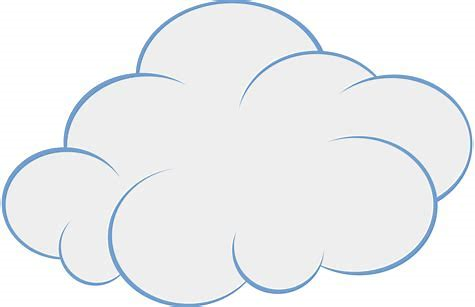
\includegraphics[width=4cm]{figs/cloud.png}};
	\node at(4,-0.5) [color=blue]{Key Space};
	
	
	\fill[ball color=red!60] (3,0.5) circle (0.1)node(x)[above,right]{$x$};
	\fill[ball color=red!60] (2.5,-0.2) circle (0.1)node(y)[above,right]{$y$};
	
	\foreach \y in{2,1.5,-1.5,-2}:
	\draw (-4,\y-0.25) rectangle (-3,\y+0.25); 
	\draw (-4,-0.25) rectangle node(k){ } (-3,0.25); 
	\draw (-4,0.25) rectangle node{$\cdots$} (-3,1.25); 
	\draw (-4,-0.25) rectangle node{$\cdots$} (-3,-1.25); 
	\node at(-5,2){$E\left[0\right]$};
	\node at(-5,1.5){$E\left[1\right]$};		
	\node at(-5,-2){$E\left[m-1\right]$};
	\node at(-5,0){$E\left[{\color{red}k}\right]$};
	\draw [dashed,color=red,thick,->](x)--(k);
	\draw [dashed,color=red,thick,->](y)--(k);
	\pause
	\node at(0,-2) {\textbf{\color{red}It depends ...}};
	\end{tikzpicture}
\end{center}
\end{frame}

\begin{frame}
\frametitle{Model \& Assumption}
\begin{block}{Model}
	\begin{itemize}
		\item Inserting {\color{blue}$n$} keys: sequence of {\color{blue}$n$} s independent trails.
		\item Each insertion corresponds to a value from $\{0,1,\cdots,m-1\}$.
	\end{itemize}
\end{block}

\pause
\begin{block}{Assumption}
	\begin{itemize}
		\item For each insertion, the result is {\color{red}Uniformly Distributed}, i.e. each value from $\{0,1,\cdots,m-1\}$ is \red{equally} picked.
	\end{itemize}
\end{block}

\pause
\shadowbox{\parbox{\textwidth}{In hashing {\color{blue}$n$} items into a hash table of size {\color{blue}$m$}, the expected number of items that hash to any one location is {\color{blue}${\color{red}\alpha}=n/m$} ({\color{red}$\alpha$}: loading factor)}}
\end{frame}

\begin{frame}
\frametitle{Empty location}
\begin{center}
	\shadowbox{
		After inserting $n$ items into $m$ locations}
\end{center}

\pause
\begin{block}{}
	\question{}{ What is the probability of a given location is {\color{red}empty}?}
	\pause
	\begin{center}
		\textbf{\color{red}	$(1-\frac{1}{m})^n$}
	\end{center}
\end{block}

\pause
\begin{block}{}
	\question{}{ What is the expected number of {\color{red}empty} locations?}
	\begin{itemize}
		\pause
		\item $X_i=\left\lbrace \begin{array}{ll}
		1&, \text{location i is empty}\\
		0&, \text{otherwise}
		\end{array}\right. $
		\pause
		\item $X=\sum\limits_{1\le i\le m}{X_i}$
		\pause
		\item $E(X)=E(\sum\limits_{1\le i\le m}{X_i})=\sum\limits_{1\le i\le m}{E(X_i)}=\sum\limits_{1\le i\le m}{(1-1/m)^n}=m(1-1/m)^n$
	\end{itemize}
\end{block}
\end{frame}
\begin{frame}
\begin{center}
	\shadowbox{
		After inserting $n$ items into a hashtable with $n$ locations}
\end{center}
\pause
\begin{block}{}
	\question{}{ What is the expected number of items in a given location?}
	\begin{center}
		\begin{itemize}
			\pause
			\item $Y_i=\left\lbrace \begin{array}{ll}
			1&,\text{the }i\text{th item in the given location}\\
			0&,\text{otherwise}
			\end{array}\right. $
			\pause
			\item $Y=\sum\limits_{1\le i\le n}{Y_i}$
			\pause
			\item $E(Y)=E(\sum\limits_{1\le i\le n}{Y_i})=\sum\limits_{1\le i\le n}{E(Y_i)}=\sum\limits_{1\le i\le n}{1/n}={\color{red}1}$
		\end{itemize}
	\end{center}
\end{block}

\pause
\begin{block}{Expected number of empty locations: $n(1-1/n)^n=n/e \approx {\color{red}0.368n}$}
\end{block}


\begin{center}
	\pause
	\textbf{\LARGE{PARADOX?}}
	
	\pause
	\fbox{\teal{collisions!}}
\end{center}
\end{frame}
\begin{frame}[t]
\frametitle{Expected number of collisions}
\begin{center}
	\shadowbox{
		After inserting $n$ items into $m$ locations}
	\begin{block}{}
		\question{}{ What is the expected number of collisions?}
		\pause
		\[
			\begin{array}{ll}
				E(\text{collisions})&=n-E(\text{occupied locations})\\\\
			\pause	&=n-\left(m-E(\text{empty locations})\right)\\\\
			\pause	&=n-\left(m-m\left(1-1/m\right)^n\right)\\\\
					&=n-m+m\left(1-1/m\right)^n
			\end{array}
		\]
	\end{block}
	\pause
	\begin{block}{Example:}
		When	$n=100, m=100$,  then $E(\text{collision})\approx37$
	\end{block}
\end{center}
\end{frame}

\begin{frame}[t]
\begin{center}
	\shadowbox{
		After inserting $n$ items into $m$ locations}
\begin{block}{}
	\question{}{What is the expected number of items needed to fullfill  all $m$ locations?}
	\begin{columns}
		\begin{column}{0.8\linewidth}
			\begin{itemize}
				\onslide<2->{\item $X_i$: the number of items to be added to increase the number of occupied locations from $i-1$ to $i$.}
				\onslide<3->{\item Given $i-1$ occupied locations, \onslide<5->{the success probability  for each trial is $(m-i+1)/m$}}
				\onslide<6->{\item Thus, $E(X_i)=m/(m-i+1)$}
				
				\onslide<7->{
				\[
				\begin{array}{ll}
				E(X)
				&=\sum\limits_{i=1}^{m}{E(X_i)}=\sum\limits_{i=1}^{m}{m/(m-i+1)}\\\vspace{0.2cm}
				&=m\sum\limits_{i=1}^{m}{1/(m-i+1)}\\\vspace{0.2cm}
				&=m\sum\limits_{j=1}^{m}{1/j}={\color{red}\Theta(m\lg{m})}
				\end{array}
				\]}
			\end{itemize}
		\end{column}
		\begin{column}{0.2\linewidth}
			\begin{center}
				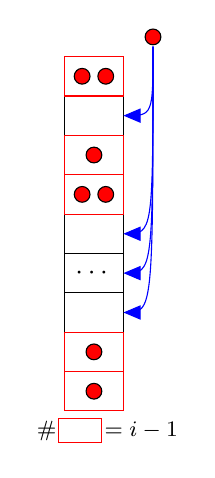
\begin{tikzpicture}[scale=0.5]
				
				
				\onslide<3->{
					\foreach \y in {-4,-3,...,4}{
						\draw (-0.75,\y-0.5) rectangle (0.75,\y+0.5);
					}
					\node at (0,-1) {$\cdots$};
					\foreach \y in {-4,-3,2}{
						\draw [color=red](-0.75,\y-0.5) rectangle (0.75,\y+0.5);
						\filldraw [fill=red](0,\y) circle (0.2cm);
					}
					\foreach \y in {1,4}{
						\draw [color=red](-0.75,\y-0.5) rectangle (0.75,\y+0.5);
						\foreach \x in{-0.3,0.3}{
							\filldraw [fill=red](\x,\y) circle (0.2cm);
						}
					}
					\node at(-1.2,-5) {\footnotesize{$\#$}};
					\draw [color=red](-0.9,-5.3) rectangle (0.2,-4.7);	
			
					\node [xshift=0.6cm]at(0,-5) {\footnotesize{$=i-1$}};
				}
				\onslide<4->{
					\filldraw [fill=red](1.5,5) circle (0.2cm)node(n1){};
				
					\foreach \y in {3,0,-1,-2}{
						\draw [color=blue,->,>=triangle 45] (n1)..controls (1.5,\y)..(0.75,\y);
					}
				}
				\end{tikzpicture}
			\end{center}
		\end{column}
	\end{columns}
	
\end{block}
\end{center}
\end{frame}

\section{Hash Functions}
\begin{frame}
\frametitle{Hashing: the idea}
\begin{center}
	\begin{tikzpicture}
	\node (a)[color=black, draw,rectangle,fill=gray] at(-0.5,0) {Hash Function} ;
	\node at (-0.5,1.5) [fill= yellow,text width=4cm]{\footnotesize{
			\begin{itemize}
			\item Index distribution
			\item Collision handling
			\end{itemize}
		}
	};
	\node (b) at (4,0){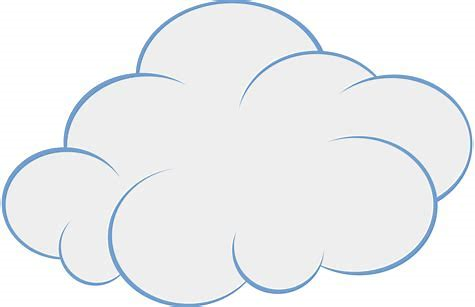
\includegraphics[width=4cm]{figs/cloud.png}};
	\node at(4,-0.5) [color=blue]{Key Space};
	\node at (4,2) [fill= yellow,text width=4cm]{\footnotesize{Very large, but only a small part is used in an application at a certain time.}};
	
	\fill[ball color=red!60] (3,0.5) circle (0.1)node(x)[above,right]{$x$};
	\foreach \y in{2,1.5,-1.5,-2}:
	\draw (-4,\y-0.25) rectangle (-3,\y+0.25); 
	\draw (-4,-0.25) rectangle node(k){ } (-3,0.25); 
	\draw (-4,0.25) rectangle node{$\cdots$} (-3,1.25); 
	\draw (-4,-0.25) rectangle node{$\cdots$} (-3,-1.25); 
	\node at(-5,2){$E\left[0\right]$};
	\node at(-5,1.5){$E\left[1\right]$};		
	\node at(-5,-2){$E\left[m-1\right]$};
	\node at(-5,0){$E\left[{\color{red}k}\right]$};
	\node at (-4,3) [fill= yellow]{\footnotesize{In feasible size}};
	\draw [dashed,color=red,thick,->](x)--(a);
	\draw [dashed,color=red,thick,->](a)--(k);
	
	\pause
	\node at(0,-2) {{\color{red} Hash Function} is IMPORTANT!};
	\end{tikzpicture}
\end{center}
\end{frame}

\begin{frame}
\frametitle{Two typical hash functions}
 \begin{block}{\textbf{\color{red} Division Method}: map a key $k$ into one of $m$ slots by taking the remainder of $k$ divided by $m$.}
 	\[
 	h(k)=k\mod m
 	\]
 \end{block}

 \begin{block}{\textbf{\color{red} Multiplication Method}:}
	\begin{itemize}
		\item \textbf{\color{blue}Step-1}: multiply the $k$ by a constant $A$ in the range $0<A<1$ and extract the \textbf{\color{blue} fractional part} of $kA$.
		\item \textbf{\color{blue}Step-2}: multiply the \textbf{\color{blue} fractional part}  by $m$.
	\end{itemize}
\end{block}
\end{frame}

\begin{frame}
\frametitle{Two typical hash functions}
\fbox{\parbox{\linewidth}{\textbf{\color{red} Division Method}: map a key $k$ into one of $m$ slots by taking the remainder of $k$ divided by $m$:
	\[
	h(k)=k\mod m
	\]
}}
	\pause
	\question{}{Why should we avoid $m=2^p$?}
	\
	\begin{itemize}
		\pause
		\item  Since if $m=2^p$, then $h(k)$ is just \teal{the $p$ lowest-order bits of $k$}.
		\pause
		\item  Unless we know that \teal{all low-order $p$-bit patterns are equally likely}, we are better off designing the hash function to \teal{depend on all the bits of the key}.
	\end{itemize}

\begin{block}{}
	\pause
	\shadowbox{\parbox{\textwidth}{A \textbf{\color{blue}prime} {\color{green}not too close to} an exact power of 2 is often a good choice for $m$. }}

	Exercise 11.3-3 
\end{block}
	

\end{frame}

\begin{frame}
\frametitle{Two typical hash functions}
\fbox{\parbox{\linewidth}{
 \textbf{\color{red} Multiplication Method}:
	\begin{itemize}
		\item \textbf{\color{blue}Step-1}: multiply the $k$ by a constant $A$ in the range $0<A<1$ and extract the \textbf{\color{blue} fractional part} of $kA$.
		\item \textbf{\color{blue}Step-2}: multiply the \textbf{\color{blue} fractional part}  by $m$
	\end{itemize}
	\[
	h(k)=\lfloor m(kA\mod 1)\rfloor
	\]
}}
	\pause
	\question{}{Why do we usually choose {\color{blue}$m=2^p$}?}
	\pause
	\begin{center}
		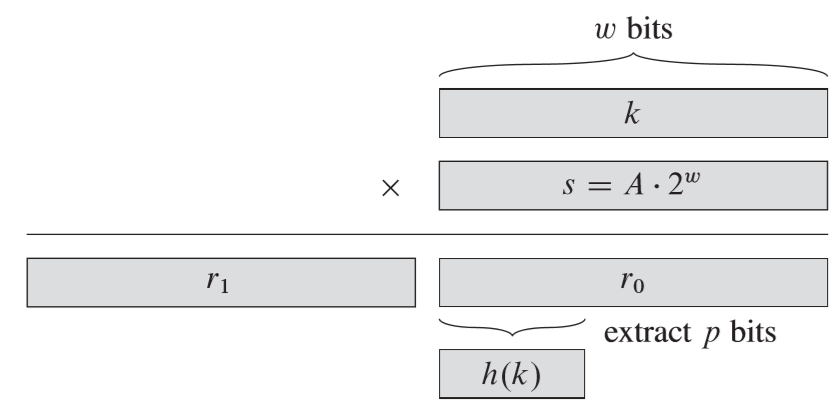
\includegraphics[width=.5\textwidth]{figs/multiplication_hashing_function.png}
	\end{center}
\end{frame}
\section{Collision Resolution}

\begin{frame}
\frametitle{Collision}
\begin{center}
	\begin{tikzpicture}
	\filldraw [fill=gray](-2,-1) rectangle (1,1);
	\node (a)[color=black] at(-0.5,0) {Hash Function} ;
	
	\node (b) at (4,0){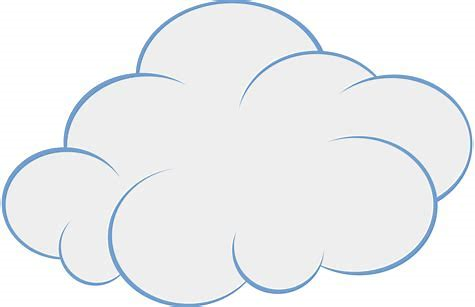
\includegraphics[width=4cm]{figs/cloud.png}};
	\node at(4,-0.5) [color=blue]{Key Space};
	
	
	\fill[ball color=red!60] (3,0.5) circle (0.1)node(x)[above,right]{$x$};
	\fill[ball color=red!60] (2.5,-0.2) circle (0.1)node(y)[above,right]{$y$};
	
	\foreach \y in{2,1.5,-1.5,-2}:
	\draw (-4,\y-0.25) rectangle (-3,\y+0.25); 
	\draw (-4,-0.25) rectangle node(k){ } (-3,0.25); 
	\draw (-4,0.25) rectangle node{$\cdots$} (-3,1.25); 
	\draw (-4,-0.25) rectangle node{$\cdots$} (-3,-1.25); 
	\node at(-5,2){$E\left[0\right]$};
	\node at(-5,1.5){$E\left[1\right]$};		
	\node at(-5,-2){$E\left[m-1\right]$};
	\node at(-5,0){$E\left[{\color{red}k}\right]$};
	\draw [dashed,color=red,thick,->](x)--(k);
	\draw [dashed,color=red,thick,->](y)--(k);
	
	\end{tikzpicture}
\end{center}
\end{frame}

\begin{frame}
\frametitle{Collision Resolution}
\begin{columns}
	\begin{column}{0.6\textwidth}
		\begin{center}
			\begin{block}{\textbf{Chaining (Closed Addressing)}}
				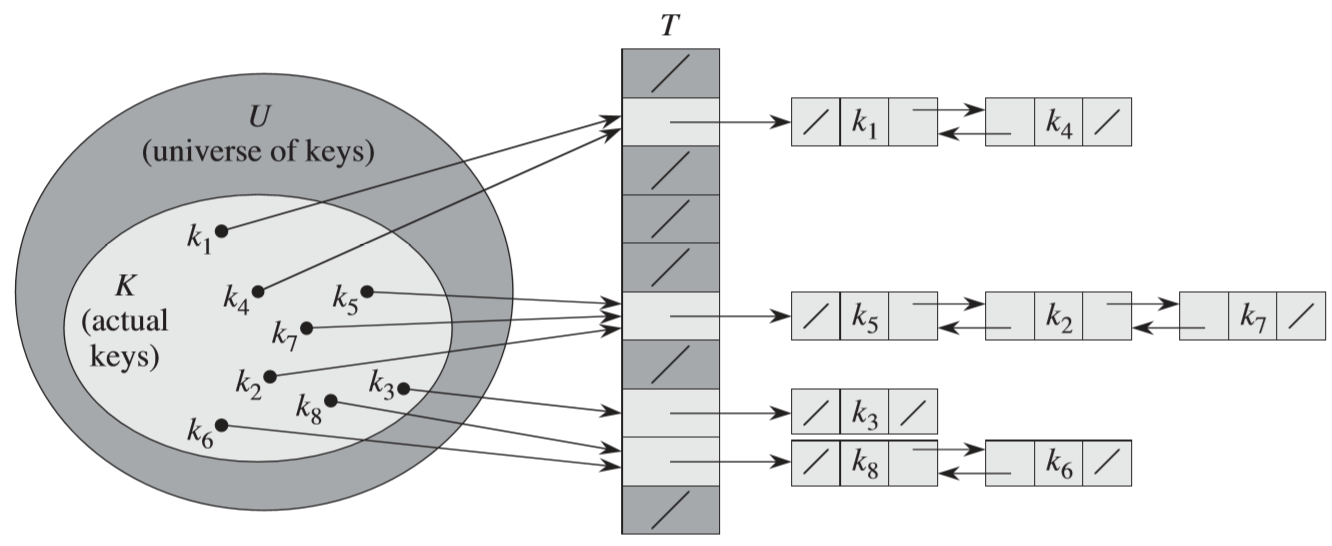
\includegraphics[width=\textwidth]{figs/cr_chaining.png}
			\end{block}
		\end{center}
	\end{column}
	\begin{column}{0.35\textwidth}
		
			\begin{block}{\textbf{Open Addressing}}
				\begin{center}
				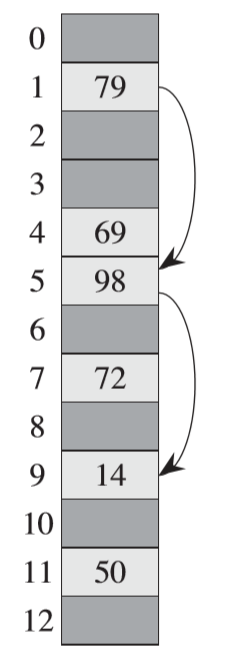
\includegraphics[width=0.25\textwidth]{figs/cr_open_addressing.png}
				
				\end{center}
			\end{block}
	\end{column}
\end{columns}
\end{frame}
\subsection{Chaining}
\begin{frame}
\frametitle{Collision Resolution by Chaining}
\begin{center}
\begin{tikzpicture}
\node at (0,0) {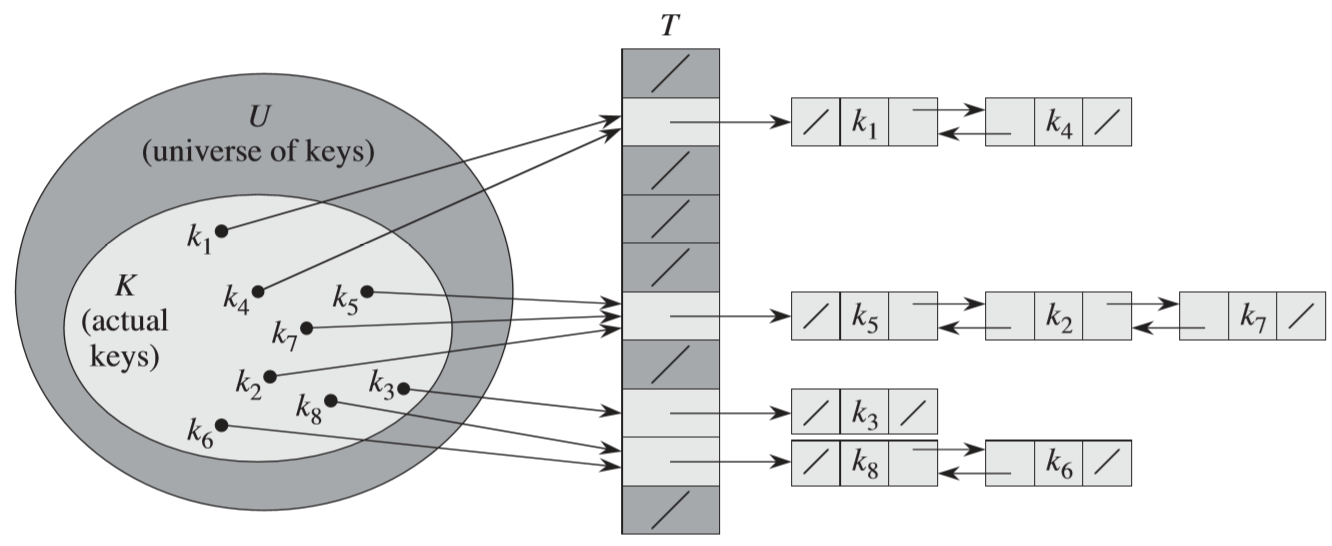
\includegraphics[width=0.7\textwidth]{figs/cr_chaining.png}};
\node at (0,-3.6) {\fbox{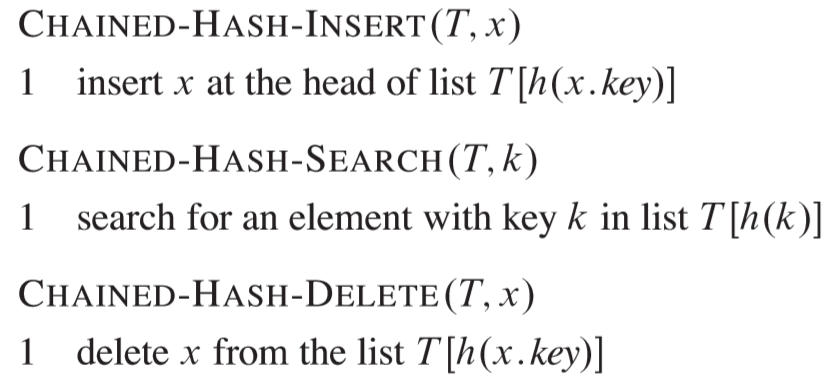
\includegraphics[width=0.6\textwidth]{figs/cr_chaining_procedure.png}}};
\pause
\draw [color=red,thick](-1,-2.8) rectangle +(0.7,0.4);
\end{tikzpicture}



\end{center}
\end{frame}

\begin{frame}
\frametitle{Collision Resolution by Chaining: Unsuccessful Search}

\question{}{What is the average cost of an \textbf{unsuccessful} search?}
\begin{block}{}
	\begin{center}
		\pause
		\shadowbox{
			\begin{tikzpicture}
				\node at (0,0) {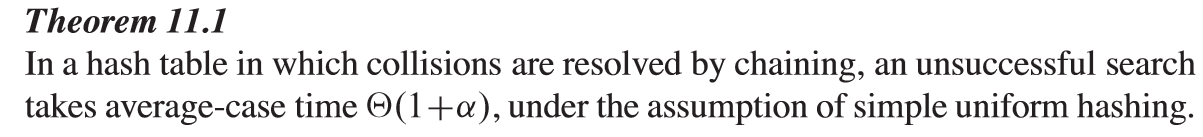
\includegraphics[width=.9\textwidth]{figs/theorem-11-1.png}};
				\draw [color=red,thick](0.4,-0.5) rectangle +(5,0.3);
			\end{tikzpicture}
		}
		
	
	\pause	
	
	\shadowbox{	\parbox{0.7\textwidth}{
		For $j=0,1,2,...,m-1$, the average length of the list at $E[j]$ is $n/m=\alpha$.
	}}
	\begin{itemize}
		\pause
		\item Any key that is not in the table is \textbf{\blue{equally}} likely to hash to any of the $m$ addresses. 
		\pause
		\item The \textbf{\blue{average cost}} to determine that the key is not in the list $E[h(k)]$ is the cost to search to the end of the list, which is $\alpha$.
		\pause
		\item Total cost is {$\Theta(\textcolor{red}{1}+{\color{blue}\alpha})$}
	\end{itemize}
	\end{center}
\end{block}
\begin{center}
\end{center}
\end{frame}

\begin{frame}
\frametitle{Collision Resolution by Chaining: Successful Search}
\question{}{ What is the average cost of an \textbf{successful} search?}
\begin{block}{}
	\begin{center}	
		\pause
		\shadowbox{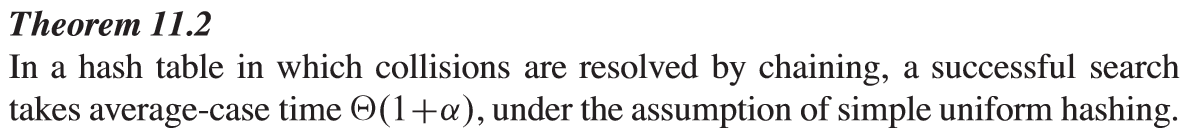
\includegraphics[width=.9\textwidth]{figs/theorem-11-2.png}}
		\begin{itemize}
			\pause\item \teal{$x_i$}: the $i$th element inserted into the table.
			\pause\item The probability of that \teal{$x_i$} is searched is $1/n$.
			\pause\item For a specific \teal{$x_i$}, the number of elements examined in a successful search is $\textcolor{red}{t}+1$
			\begin{itemize}
				\pause\item $\textcolor{red}{t}$: the number of elements inserted into the same list as \teal{$x_i$}, \textbf{after} \teal{$x_i$} has been inserted.
				\pause\item The probability of that $x_j$ is inserted into the \textbf{same} list of \teal{$x_i$} is $1/m$.
				\pause\item The \textbf{\color{blue}expected number of elements examined} for a successful search of \teal{$x_i$} is {$(\textcolor{blue}{1}+\textcolor{red}{\sum\limits_{j=i+1}^{n}{\frac{1}{m}}})$}
			\end{itemize}
		\end{itemize}
	\end{center}
\end{block}
\end{frame}

\begin{frame}
\frametitle{Collision Resolution by Chaining: Successful Search}
\question{}{What is the average cost of a \textbf{successful} search?}
\begin{block}{}
	\begin{center}	
		\begin{itemize}
			\item  Average \textbf{\color{blue}number of elements examined} for an successful search is \[
			\begin{array}{ll}
			\frac{1}{n}\sum\limits_{i=1}^{n}{(\textcolor{blue}{1}+\textcolor{red}{\sum\limits_{j=i+1}^{n}{\frac{1}{m}}})}
			\pause&=1+\frac{1}{n\textcolor{red}{m}}{(\textcolor{red}{\sum\limits_{j=i+1}^{n}{1}})}\\\vspace{0.2cm}
			\pause&={1}+\frac{1}{nm}{({\sum\limits_{i=1}^{n}{n-i}})}\\\vspace{0.2cm}
			\pause&={1}+\frac{1}{nm}{(n^2-{\sum\limits_{i=1}^{n}{i}})}\\\vspace{0.2cm}
			\pause&={1}+\frac{1}{nm}{(n^2-\frac{n(n+1)}{2})}\\\vspace{0.2cm}
			&={1}+\frac{n}{2m}-\frac{n}{2nm}\\\vspace{0.2cm}
			&={1}+\alpha-\frac{\alpha}{2n}
			\end{array}\]
		\end{itemize}
		\pause
		\item  Average \textbf{\color{blue}cost} for a successful search is ${\blue{\textbf{2}}}+\alpha-\frac{\alpha}{2n}=\Theta(1+\alpha)$
	\end{center}
\end{block}
\end{frame}


\begin{frame}[fragile]
\frametitle{Collision Resolution by Chaining: Example}
\begin{block}{JAVA 7 HashMap}
	
	\begin{columns}
		\begin{column}{0.7\textwidth}
\begin{lstlisting}[style=styleJ]
static int hash(int h) {
    h^= (h>>>20)^(h>>>12);
    return h^(h>>>7)^(h>>>4);
}
\end{lstlisting}
			\begin{itemize}
				\item In \red{Java 7}, after calculating hash from hash function, if more then one element has same hash than they are searched by linear search, so it's complexity is $O(n)$.
				
				\item In \red{Java 8}, that search is performed by \textbf{\teal{binary search}} so the complexity will become $\log{n}$.
			\end{itemize}
		\end{column}
		\begin{column}{0.25\textwidth}
			
\includegraphics[width=\linewidth]{figs/java7.png}
		\end{column}
	\end{columns}
\end{block}
\end{frame}

\subsection{Open Addressing}
\begin{frame}
\frametitle{Open Addressing}
\begin{columns}
	\begin{column}{0.2\linewidth}
		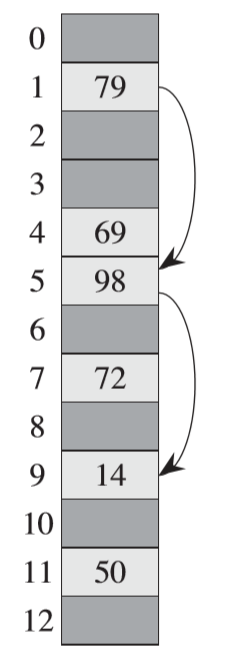
\includegraphics[width=\linewidth]{figs/cr_open_addressing.png}
	\end{column}
	\begin{column}{0.85\linewidth}
		\begin{itemize}
			\item All elements are stored in the hash table, \textbf{no linked list is used}. So, $\alpha\le 1$.
		
			\pause
			\item Collision is settled by ``\textbf{\color{red}rehashing}'':
			\begin{itemize}
				\pause\item 	A function used to get \textbf{a new hashing address for each collided address}
				\pause\item The hash table slots are probed successively, until a valid location is found.
			\end{itemize} 
		
			\pause
			\item The \textbf{\teal{probing sequence}} can be seen as a \textbf{\teal{permutation}} of $(0,1,2,\cdots, m-1)$$\rightarrow$$\left\langle h(k,0), h(k,1),\cdots, h(k,m-1)\right\rangle $
			
		\end{itemize}
	\end{column}
\end{columns}
\end{frame}


\begin{frame}
\frametitle{Open Addressing: Commonly Used Probings}

\begin{block}{\textbf{\color{red}Linear Probing}: (\textbf{\color{blue}primary clustering} may occur)}
Given an auxiliary hash function $h'$, the hash function is: 
	\[h(k,i) = (h'(k)+i)\mod {m},  (i=0,1,...,m-1)\]
\end{block}
\pause
\begin{block}{\textbf{\color{red}Quadratic Probing}: (\textbf{\color{blue}secondary clustering} may occur)}
Given auxiliary function $h'$ and nonzero auxiliary constant $c_1$ and $c_2$, the hash function is: 
	\[h(k,i) = (h'(k)+c_1i+ c_2i^2) \mod m,   (i=0,1,...,m-1)\]
\end{block}
\pause
\begin{block}{\textbf{\color{red}Double Hashing}:}
Given auxiliary functions $h_1$ and $h_2$, the hash function is: 
\[h(k,i) = (h_1(k)+ ih_2(k)) \mod m, (i=0,1,...,m-1)\]
\end{block}	
\end{frame}



\begin{frame}
\frametitle{Linear Probing: an Example}
\begin{center}
	\begin{tikzpicture}
	\node (b) at (4,2){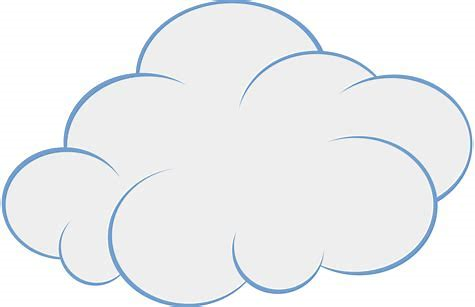
\includegraphics[width=4cm]{figs/cloud.png}};	

	
	\foreach \y in{0,1,...,7}:{
		\draw (-4.5,\y*0.5-0.25) rectangle (-3,\y*0.5+0.25); 
		\node at(-5,3.5-\y*0.5){\y};	
	}
	\node at(-3.75,3.5)[color=blue]{1776};
	\node at(-3.75,2)[color=blue]{1055};
	\node (l4) at(-3.75,1.5)[color=blue]{1492};
	\node (l6)at(-3.75,0.5)[color=blue]{1918};
	\node at(2,4) {\shadowbox{Hasing function: $h(x)=5x\mod 8$}};
	\node at(2,0) {\shadowbox{Rehasing function: $rh(j)=(j+1)\mod 8$}};	
	
	%1812
	\pause
	\fill[ball color=red!60] (3,2.5) circle (0.1)node(n1812)[above,right,color=red!80!black!80!]{$1812$};
	\pause
	\draw [->,dashed,color=red,thick](n1812)--node[above]{hashing}(l4)[right=1cm];
	
	
	\pause
	\node (l5)at(-3.75,1)[color=white]{\textbf{1812}};
	\draw [->,dashed,color=red,thick](l4)[left]..controls (-5,1.5) and (-5,1.0)..(l5)[left];
	\node at(-5.5,1.25)[color=red]{rehashing};
	\pause
	\node at(-3.75,1)[color=red!80!black!80!]{\textbf{1812}};
	
	%1945
	\pause
	\fill[ball color=red!60] (2.5,1.8) circle (0.1)node(n1945)[above,right,color=green!80!black!80!]{$1945$};
	
	\pause
	\draw [->,dashed,color=green,thick](n1945)--node[below]{hashing}(l5)[right=1cm];
	\pause
	\draw [->,dashed,color=green,thick](l5)[right]..controls (-2.25,1) and (-2.25,0.5)..(l6)[right];
	\node (l7) at(-3.75,0)[color=white]{\textbf{1945}};
	\pause
	\draw [->,dashed,color=green,thick](l6)[right]..controls (-2.25,0.5)and(-2.25,0)..(l7)[right];
	\node at(-2,0.5)[color=green]{rehashing};
	\pause
	\node  at(-3.75,0)[color=green!80!black!80!]{\textbf{1945}};

	
	
	
	
	
	\end{tikzpicture}
\end{center}
\end{frame}

\begin{frame}
\frametitle{Open Addressing: Commonly Used Probings}
\question{}{How to evaluate the \textbf{goodness} of a probing?}
\begin{block}{}
\begin{center}
	
\pause
\textbf{\color{red}Assumption}

\shadowbox{\parbox{0.8\linewidth}{Each key is \textbf{equally} likely to have any of the $m!$ permutations of $(1,2,\cdots,m-1)$ as its probe sequence.
}}

\begin{itemize}
	\pause\item Both linear and quadratic probing have only {\color{blue}$m$ distinct probe sequences}, as determined by the first probe.
	\begin{center}
		$h(k,i) = (h'(k)+i)\mod {m},  (i=0,1,...,m-1)$
		
		$h(k,i) = (h'(k)+c_1i+ c_2i^2) \mod m,   (i=0,1,...,m-1)$
	\end{center}
	\pause\item Double hashing improves over linear or quadratic probing in that {\color{blue}$\Theta(m^2)$ probe sequences} are used.
	\[h(k,i) = (h_1(k)+ ih_2(k)) \mod m, (i=0,1,...,m-1)\]
\end{itemize}
\end{center}
\end{block}
\end{frame}

\begin{frame}
\frametitle{Open Addressing: Deleting Element}
\question{}{Why Open Addressing is not suitable for situations where items might be deleted?}
	\begin{center}
		
		\begin{itemize}
			\pause\item The probing chain might be broken if an item is deleted.
			\pause \item How to deal with it?
		\end{itemize}
	\end{center}
\end{frame}

\begin{frame}
\frametitle{Open Addressing: Unsuccessful Search}
\question{}{Assuming uniform hashing, what is the average number of probes in an \textbf{unsuccessful} search?}
\begin{center}
	\pause
	\shadowbox{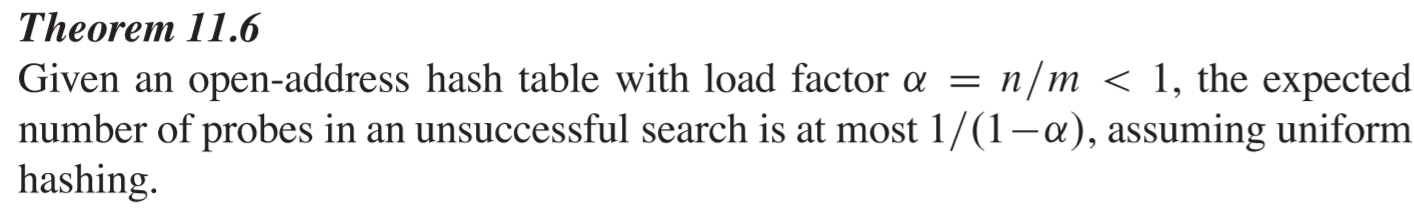
\includegraphics[width=0.9\linewidth]{figs/theorem-11-6.png}}
\end{center}
\begin{itemize}
	\pause
	\item {\color{blue}$X$}: the number of probes made in an \textbf{unsuccessful} search
	\pause
	\[
	\begin{array}{ll}
	E(X)&=\sum\limits_{i=0}^{\infty}{i\cdot Pr(X=i)}\\\vspace{0.2cm}
	&=\sum\limits_{i=0}^{\infty}{i\cdot( Pr(X\ge i)-Pr(X\ge i+1))}\\\vspace{0.2cm}
	&={\color{blue}\sum\limits_{i=1}^{\infty}{Pr(X\ge i)}}
	\end{array}
	\]
\end{itemize}
\end{frame}

\begin{frame}
\frametitle{Open Addressing: Unsuccessful Search}
\question{}{How to compute $Pr(X\ge i)$?}
\begin{itemize}
	\pause\item $A_i$: the $i$th probe occurs at an \teal{occupied} slot
	\pause\item $X\ge i=A_1\cap A_2\cap\cdots\cap A_{i-1}$

\end{itemize}
\begin{proof}[]
	\pause
	{\footnotesize\[
	\begin{array}{ll}
	Pr(X\ge i)&=Pr(A_1\cap A_2\cap\cdots\cap A_{i-1})\\\vspace{0.2cm}
	&=Pr(A_1)\cdot Pr(A_2|A_1)\cdot Pr(A_3|A_1\cap A_2)\cdots Pr(A_{i-1}|A_1\cap A_2\cap\cdots\cap A_{i-2})\\\vspace{0.2cm}
	&=\frac{n}{m}\cdot\frac{n-1}{m-1}\cdots\frac{n-i+2}{m-i+2}\\\vspace{0.2cm}
	&\le (\frac{n}{m})^{i-1}\\\vspace{0.2cm}
	&=\alpha^{i-1}
	\end{array}
	\]
	}
	\pause
	Then, 
		$\begin{array}{ll}
		E(x)={\color{blue}\sum\limits_{i=1}^{\infty}{Pr(X\ge i)}}
		\le\sum\limits_{i=1}^{\infty}{\alpha^{i-1}}
		=\le\sum\limits_{i=0}^{\infty}{\alpha^{i}}=\blue{\frac{1}{1-\alpha}}		
	\end{array}$

\end{proof}
\end{frame}

\begin{frame}
\frametitle{Open Addressing: Inserting an Element}
\question{}{What is the average cost for inserting an element into a table with load factor $\alpha$?}

\begin{center}
	\pause
	\shadowbox{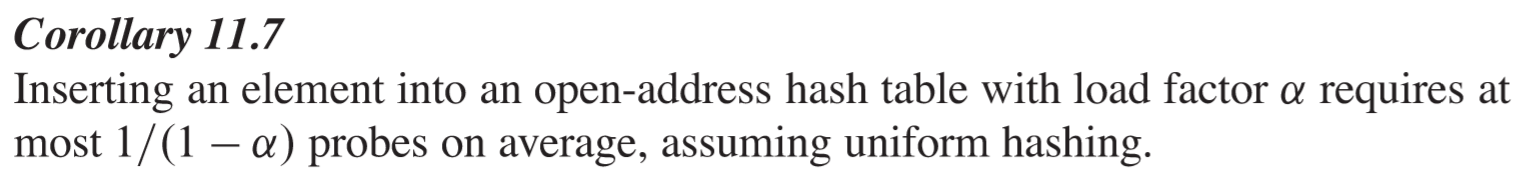
\includegraphics[width=0.9\linewidth]{figs/corollary-11-7.png}}
	\begin{proof}
		\begin{itemize}
			\item 	An element is inserted only if there is room in the table, and thus $\alpha<1$.
			\item Inserting a key requires an \teal{ unsuccessful} search followed by placing the key into the first empty slot found. 
			\item Thus, the expected number of \blue{probes} is at most $1/(1-\alpha)$ 
		\end{itemize}

	\end{proof}
\end{center}
\end{frame}

\begin{frame}
\frametitle{Open Addressing: Insertion/Unsuccessful Search}
\begin{center}
	
	\begin{tikzpicture}
	\node at(0,0){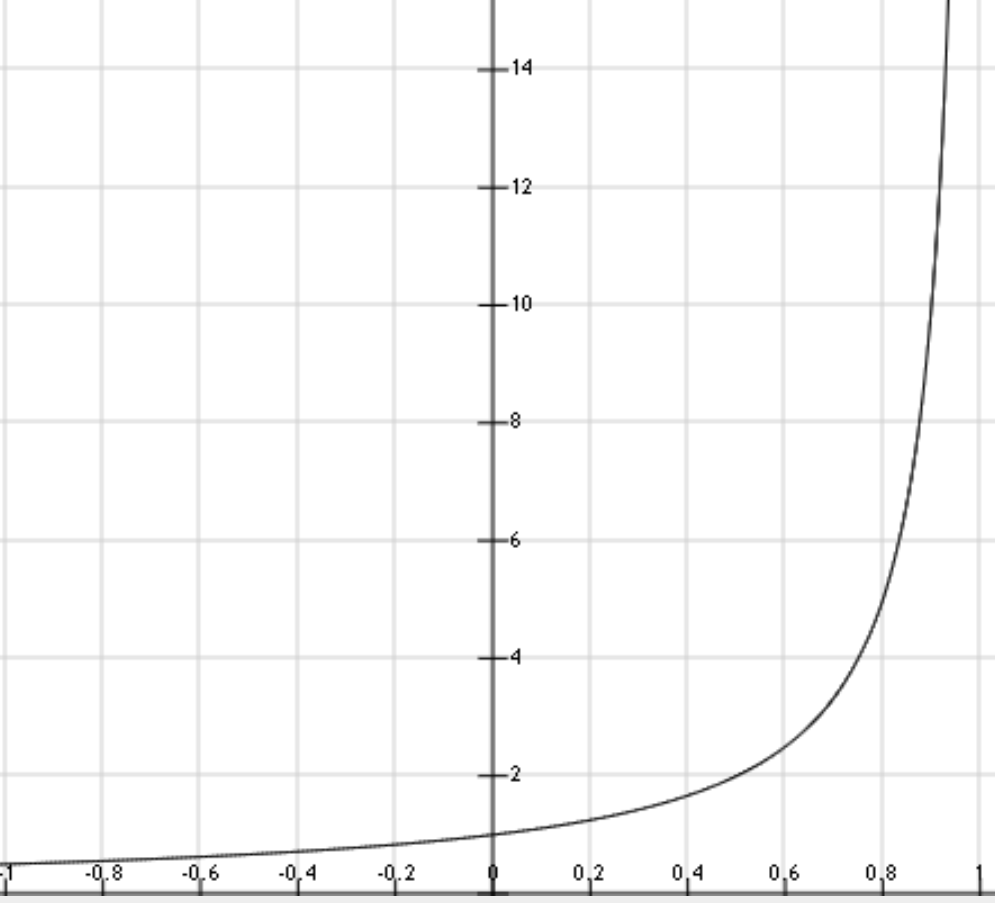
\includegraphics[width=0.5\linewidth]{figs/functiongraph1.png}};
	\filldraw [color=white](-3.6,-2.5)rectangle(-0.04,-2.2);
	\node[fill=white] at(-2,1.5){\fbox{$\frac{1}{1-\alpha}$}};				
	\end{tikzpicture}
\end{center}
\end{frame}

\begin{frame}
\frametitle{Open Addressing: Successful Search}
\question{}{What is the average number of probes in a \textbf{successful} search of an element in a table with load factor $\alpha$?}

\begin{center}
	\pause
	\shadowbox{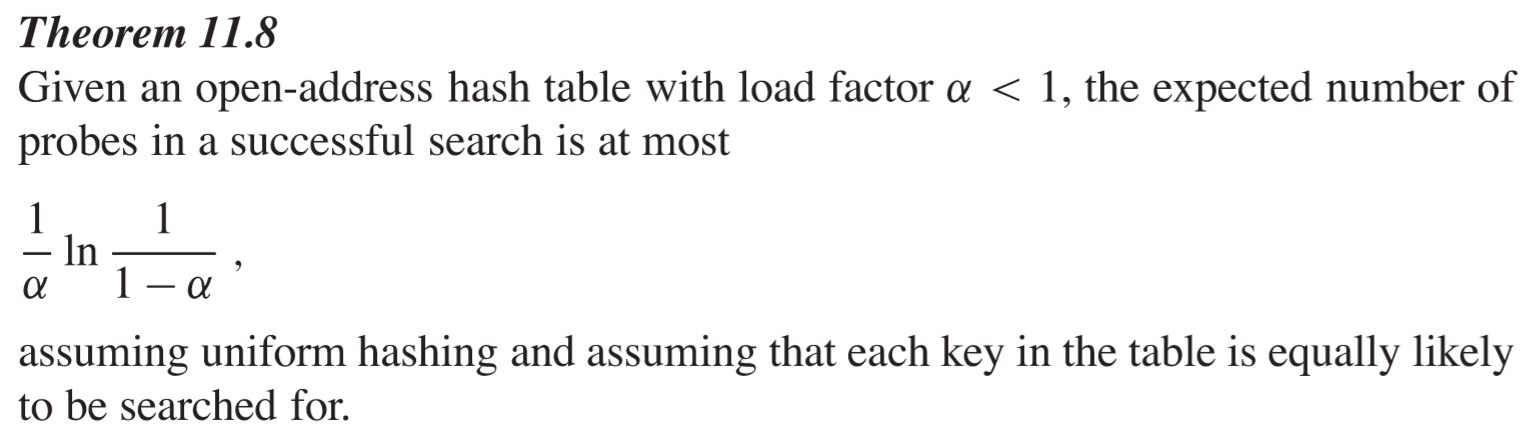
\includegraphics[width=0.9\linewidth]{figs/theorem-11-8.png}}
\end{center}
\end{frame}

\begin{frame}
\frametitle{Open Addressing: Successful Search}
\question{}{what is the average number of probes in a successful search for an element in a table with load factor $\alpha$?}

\begin{center}
\begin{proof}
	\begin{itemize}
		\pause\item A \textbf{\teal{search}} for a key $k$ reproduces the \textbf{same probe sequence} as when the element with key $k$ was \textbf{\teal{inserted}}.
		\pause\item If $k$ is the (i+1)st key inserted into the table, the expected number of probes in a search for $k$ is at most $1/(1-\blue{i/m})=m/(m-i)$
		\pause\item The expected number of probes is:
		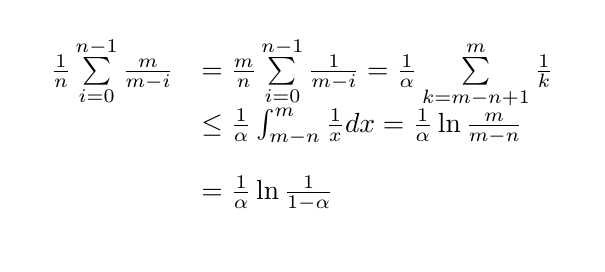
\begin{tikzpicture}
		\node at(0,0){
			$
			\begin{array}{ll}
			\frac{1}{n}\sum\limits_{i=0}^{n-1}{\frac{m}{m-i}}
			&=\frac{m}{n}\sum\limits_{i=0}^{n-1}{\frac{1}{m-i}}
			=\frac{1}{\alpha}\sum\limits_{k=m-n+1}^{m}{\frac{1}{k}}\\\vspace{0.4cm}
			&\le \frac{1}{\alpha}\int_{m-n}^{m}\frac{1}{x}dx=\frac{1}{\alpha}\ln{\frac{m}{m-n}}\\\vspace{0.3cm}
			&=\frac{1}{\alpha}\ln{\frac{1}{1-\alpha}}
			\end{array}
			$
		};
		
		\end{tikzpicture}

	\end{itemize}
\end{proof}
\end{center}
\end{frame}


\begin{frame}
\frametitle{Open Addressing: Successful Search}
\begin{center}
	
\begin{tikzpicture}
\node at(0,0){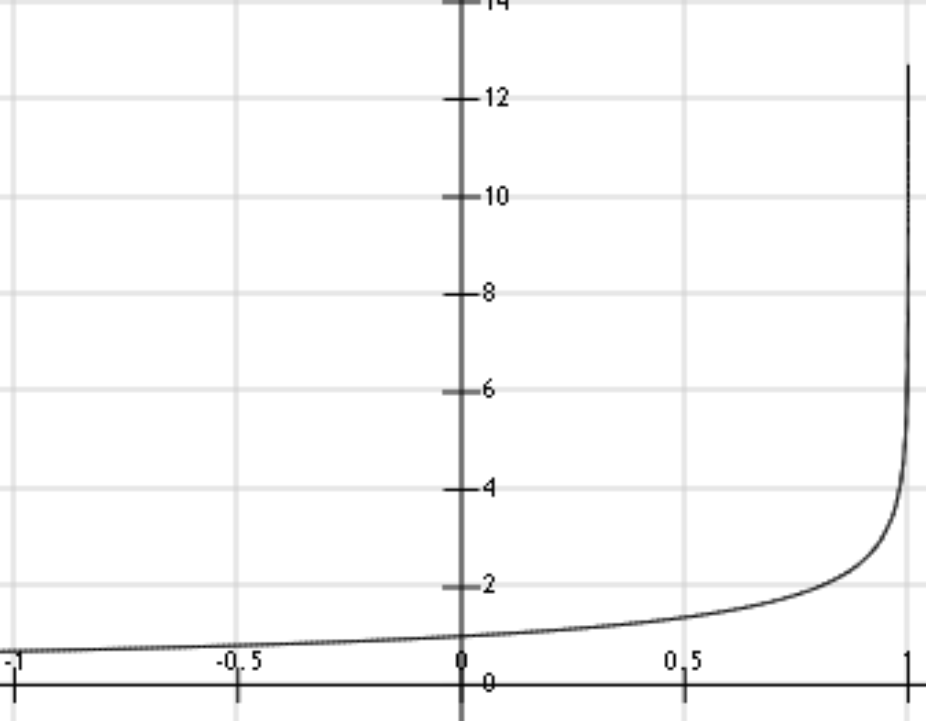
\includegraphics[width=0.5\linewidth]{figs/functiongraph.png}};
\filldraw [color=white](-3.6,-2)rectangle(-0.03,-1.8);
\filldraw [color=white](-4,1.8)rectangle(4,2.5);
\node[fill=white] at(-2,1.5){\fbox{$\frac{1}{\alpha}\ln{\frac{1}{1-\alpha}}$}};
\node at(0,-3.3) {\fbox{\parbox{3.5cm}{\teal{For your reference}: 
			\begin{itemize}
			\item $\alpha=0.5$: 1.387
			\item $\alpha=0.9$: 2.559
			\end{itemize}
			
}}};
\end{tikzpicture}
\end{center}
\end{frame}

\begin{frame}
	\begin{block}{
		\begin{center}
		{\huge
			Thank You!
			
			\vspace{0.3cm}
			\textcolor[rgb]{1,0,0}	{Questions?}
		}
		\end{center}
	}
	\end{block}
	\begin{block}{}
		\begin{center}
		
			Office 819
			
			majun@nju.edu.cn
		\end{center}
	\end{block}
	\end{frame}
\end{document}